% !TeX encoding = UTF-8
\chapter{Gestensteuerung}
\thispagestyle{fancy}

Die Gestensteuerung hat die Aufgabe Handbewegungen über eine Smartphone-Kamera zu erkennen. Dabei werden zwei Richtungen erkannt und Signale zum vor- und zurückblättert von PDF-Seiten gesendet. Auf Grund der Vorlesung und Recherchen im Internet war schnell klar, dass \href{http://opencv.org/}{OpenCV} eine zweckmäßige Bibliothek darstellt. Als Qt Basis wurde die Version 5.7 und OpenCV in der Version 3.1 verwendet. Der Code für die Gestenerkennung befindet sich unter folgendem \href{https://github.com/BeckmaR/EmbeddedMultimediaSS2016/tree/master/src/handcontrol}{Link}. Hierbei wurde ein C++ Klasse "`handcontrol"' erstellt, welche in die App eingebunden ist.

\section{Auslesen von Videoframes aus einer Kamera}
Im Laufe des Projektes stellte sich heraus, dass die Einbindung der Kamera, auf den verschiedenen Plattformen Windows und Android, die größte Herausforderung darstellt. Die Windows Unterstützung wurde hauptsächlich ausgewählt, um den Algorithmus nicht umständlich auf einem Android Gerät jedes mal testen zu müssen. Die Implementierung auf der Windows-Plattform war relativ einfach, da OpenCV schon eine Funktion \href{http://docs.opencv.org/3.1.0/d8/dfe/classcv_1_1VideoCapture.html}{VideoCapture} bietet, welche einzelne Videoframes aus eine Kamera auslesen kann und diese in einer Matrix abspeichert. Diese Methode funktionierte leider nicht auf einen Android-Gerät. Hinweise: nachfolgende Funktionsweisen beziehen sich auf den Entwicklungsstand vom 20.7.2016, ggf. sind schon Bugs behoben oder neue Möglichkeiten zur Kameraauswertung hinzugekommen. Vom Autor wurden unterschiedlichste Varianten zum Auslesen der Kamera über mehrere Stunden untersucht. Von Qt werden hauptsächlich \href{http://doc.qt.io/qt-5/videooverview.html}{zwei Möglichkeiten} für das Auslesen eines VideoFrames angeboten. \href{http://doc.qt.io/qt-5/qabstractvideosurface.html}{QAbstractVideoSurface} definiert eine abstrakte C++ Klasse welche die Funktion present() beinhaltet, welcher die einzelnen Videoframes nacheinander übergeben werden. Ähnlich verhält es sich mit \href{http://doc.qt.io/qt-5/qvideoprobe.html}{QVideoProbe} wobei man hier die Verbindung über ein Connect() mit Signal und Slot hergestellt werden muss. Eine weitere Möglichkeit besteht seit Qt 5.5 darin, ein Video Filter\footnote{\label{video_filter}https://blog.qt.io/blog/2015/03/20/introducing-video-filters-in-qt-multimedia/} in QML zu verwenden und mit Hilfe der Klasse \href{http://doc.qt.io/qt-5/qabstractvideofilter.html}{QAbstractVideoFilter} die einzelnen Videoframes in C++ zu analysieren und ggf. wieder nach QML zu transformieren. Die C++ QCamera funktioniert nicht auf Android-Geräten (\href{https://bugreports.qt.io/browse/QTBUG-41194}{1},\href{http://stackoverflow.com/questions/28041741/qt-qml-camera-to-c-qimage-on-android}{2}), sodass auf das in QML integrierte Camera Objekt zurückgegriffen wird. Bei der QAbstractVideoFiler Variante konnten die Videodaten in Android nicht in den CPU-Adressraum gemappt werden. Mit QVideoProbe war dies möglich. Hierbei wird aus QML das QCamera Objekt in C++ adressierbar gemacht und mit dem QVideoProbe verbunden. Seit Qt 5.6 existiert ein VideoOutput Objekt in QML welches das Auslesen und Anzeigen von VideoFrames steuert, sodass das hier angegebene \href{http://stackoverflow.com/questions/28041741/qt-qml-camera-to-c-qimage-on-android/33238150\#33238150}{Beispiel} noch um ein VideoOutput Objekt ergänzt werden muss. Um keine größeren Unterschiede zwischen dem Algorithmus für die Windows- und der Androidversion zu haben, ist es wünschenswert beide Cameras über Qt auslesen zu lassen. Leider funktioniert der oben für Android vorgestellte Ansatz für Windows nicht. Hier ist ein Workaround mit einer C++ QCamera und dem QAbstractVideoSurface nötig, um ein QVideoFrame zu erhalten. Die neue Variante mit dem "`Video Filter"' wurde auch untersucht, hat aber nur auf ein paar Androidgeräten funktioniert \href{https://bugreports.qt.io/browse/QTBUG-47934/}{QTBUG-47934}. Anscheinend gibt es dort noch Fehler in dem Qt-Framework. Unter folgendem \href{https://wiki.qt.io/Qt_5.7_Multimedia_Backends}{Link} gibt es eine Auflistung welche Funktionen in dem Qt-Multimedia-Framework-5.7 auf den verschiedenen Plattformen aktuell funktionieren.

\subsection{Verbesserungen}
Die mit Qt 5.5 eingeführten Video Filter scheinen ein gute Weg zu sein, um VideoFrames in Qt analysieren zu können. Leider ist aktuell die Implementierung nicht auf allen Androidgeräten funktional, sodass auf ein Workaround mit QVideoProbe zurückgegriffen werden musste. Diese Variante ist aber leider nicht optimal, da sie Verzögerungen zwischen dem Aufnehmen und dem Aufruf der Funktion present() enthält\footnote{https://blog.qt.io/blog/2015/03/20/introducing-video-filters-in-qt-multimedia/\#comment-1195419}. Eine weitere Möglichkeit besteht, QML \href{http://doc.qt.io/qt-5/qml-qtquick-shadereffect.html}{ShaderEffect} mit OpenGL zu verwenden. Da die Android Kamera seine Videoframes auf der Grafikkarte in OpenGL Texture vorhält \footnote{https://blog.qt.io/blog/2015/03/20/introducing-video-filters-in-qt-multimedia/\#comment-1195414}, wäre es sinnvoll diese auch dort weiter zu verarbeiten. Das kann seit neuem mit Video Shader Objekten direkt in QML programmiert werden. Außerdem war es dem Autor über QML nicht möglich exakte Auflösungen und Frameraten einzustellen. Anscheinend ignoriert Qt gewisse Parameter auf verschiedenen Platformen oder es stehen nicht alle Einstellung zur Verfügung. Jedenfalls sind diese nicht richtig dokumentiert. Ein Problem ist außerdem, dass es vorkommen kann das Frameraten von 30 fps auf 16 fps einbrechen oder kein reproduzierbares Verhalten zeigen. Dieser Punkt konnte innerhalb der Arbeit leider nicht geklärt werden. Eine andere Möglichkeit, welche nicht weiter verfolgt wurde, wäre über Qt mit den \href{http://doc.qt.io/qt-5/qtandroidextras-module.html}{Qt Android Extras} die Androidkamera über Java Code in die Qt Anwendung einzubetten, ggf. auch über das vorhandene OpenCV Java Binding. 

\section{Handerkennungsalgorithmus}
Aus Qt liegen die QVideoFrames als RGB (Windows) und als YUV420 (Android) vor. Diese werden als erstes in Grauwertbilder umgewandelt. Bei dem Android QVideoFrame muss keine pixelweise Konvertierung durchgeführt werden, sondern es wird nur der Luminanz Y Teil des Bildes genommen. Anschließend wird das Differenzbild zwischen dem aktuellen und vorherigen Grauwertbild berechnet. Hierbei achtet OpenCV selbständig darauf, dass eine Sättigung im Zahlenbereich durchgeführt wird.

\begin{figure}[ht!]
\centering
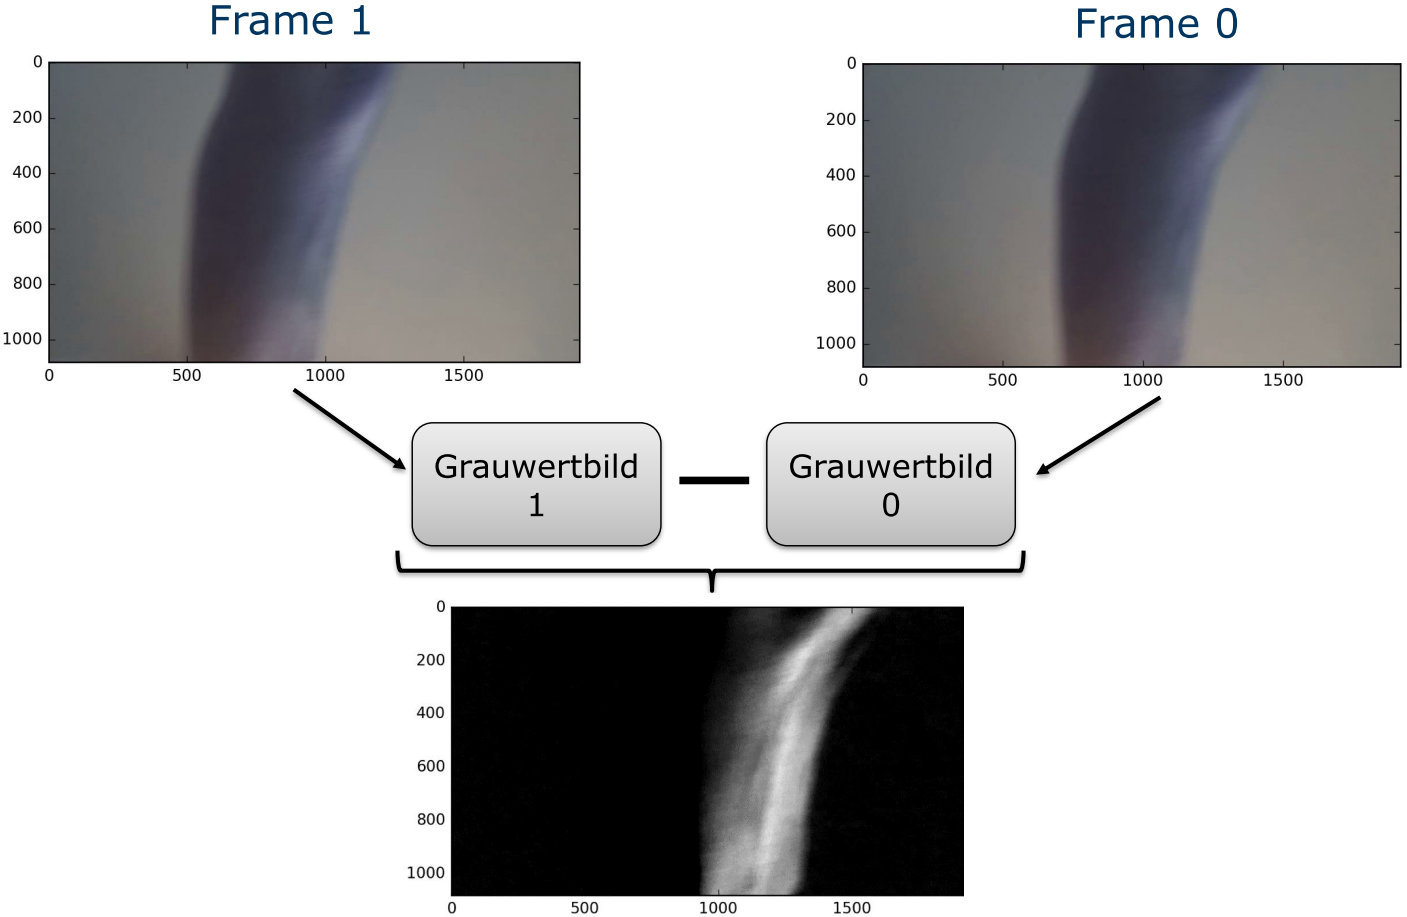
\includegraphics[angle=0,width=14cm]{handcontrol/Bilder/diff_frame1-frame0.png}
\caption{Differenzberechnung zwischen aktuellem und vorherigen Grauwertbild}
\end{figure}

Im nachfolgenden Schritt wir mit Hilfe der reduce() Funktion von OpenCV ein Mittelwert über alle Spalten gebildet. Man erhält einen Zeilenvektor wobei jeder Eintrag den Mittelwert eine Spalte repräsentiert. Hierbei kann man schnell erkennen wo sich in der Horizontalen die größten Änderungen ergeben. Das nennt der Autor Histogramm, da es die Häufigkeitsverteilung darstellt.

\begin{figure}[ht!]
\centering
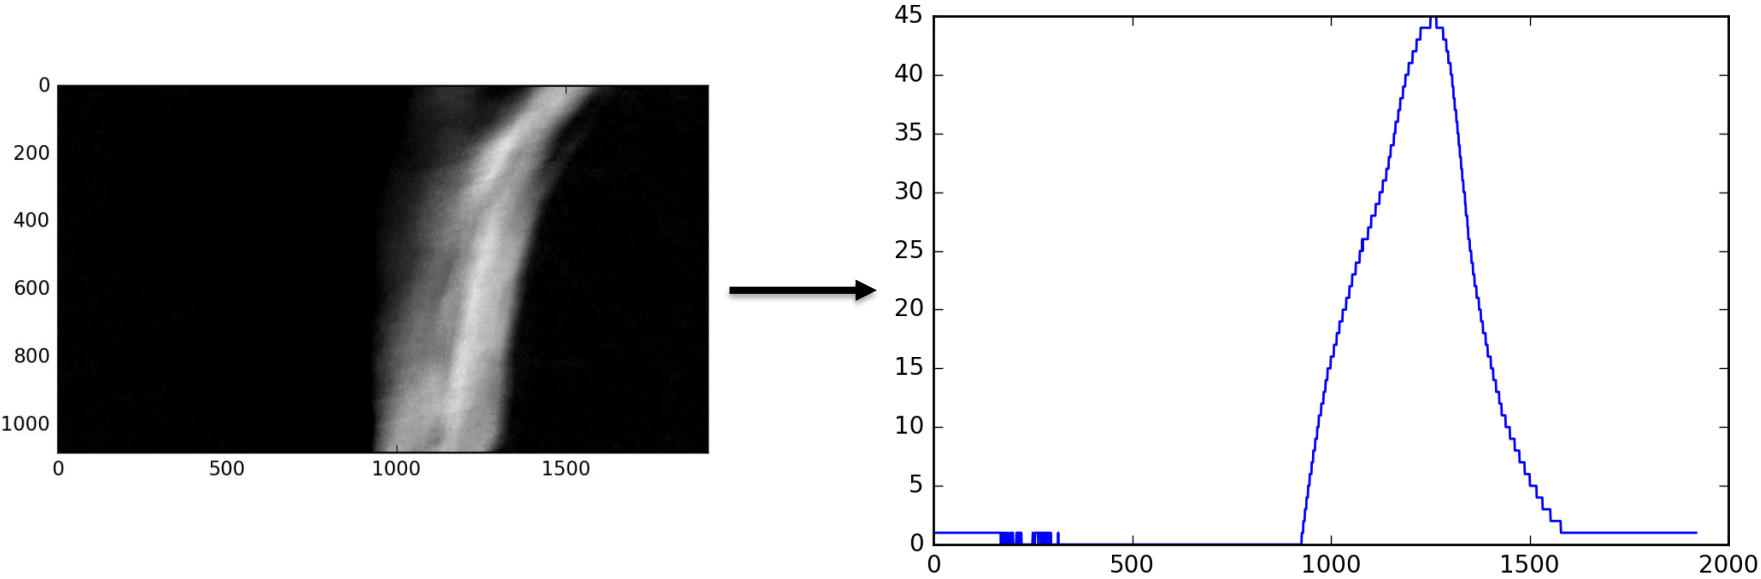
\includegraphics[angle=0,width=14cm]{handcontrol/Bilder/diff_frame_to_hist.png}
\caption{Berechnung des Histogramms über die Spalten eines Differenzbildes}
\end{figure}

Untersucht man die Verschiebung des Histogramms über die Horizontalen, kann man Handbewegungen erkennen. Hierbei wird als erstes der Schwerpunkt des Histogramms gebildet. Das geschieht mit Hilfe einer kumulierten Summe über alle Histogrammwerte. Würde man nur den maximalen Wert des Histogramms betrachten, kann bei verrauschten Bildern eine zu große Abweichung auftreten. Vor dem Berechnen des Schwerpunktes wird noch ein konstanter Faktor subtrahiert, um den ggf. existierenden Rauschteppich zu entfernen. Zur weiteren Fehlerreduktion wurden im folgenden nur diese Schwerpunkte ausgewählt, welche auch mindestens einen gewissen maximalen Histogrammwert aufweisen. Der Wert kann im Sourcecode nachgelesen werden. Um auszuwerten, ob eine PDF vor- oder zurückgeblättert werden soll, untersucht der Algorithmus zeitlich aufeinanderfolgende Schwerpunkte von Histogrammen der Differenzbilder. Er sendet ein Signal, wenn ohne Unterbrechung der Schwerpunkt eine gewisse Zeit in eine der beiden Richtungen gewandert ist. Um den GUI-Thread nicht zu überlasten und um eine flüssige Bedienung der GUI sicher zu stellen, wurde der Algorithmus in ein QThread verschoben. Der so beschriebene Algorithmus benötigt mit 30 Frames pro Sekunde auf Windows ~7ms und auf Android ~10 ms. Somit ist die Echtzeitfähigkeit gegeben. Als Alternative zum dem Differenzbild wurde auch der in OpenCV implementierte Background Substraction Algorithmus (\href{http://docs.opencv.org/3.0-rc1/d7/d7b/classcv_1_1BackgroundSubtractorMOG2.html}{BackgroundSubtractorMOG2}) untersucht. Dieser schätzt den Hintergrund über gaußsche Mischungsverhältnisse mit Mittelwert und Kovarianzmatrix. Leider benötigt der Algorithmus viel Berechnungszeit (~14 Windows und ~30 ms Android) und kratzt somit bei Android Geräten an der Echtzeitfähigkeit. Außerdem würde eine solche Implementierung zu viel Energie des Akkus verbrauchen und wurde deshalb verworfen.

\begin{figure}[ht!]
\centering
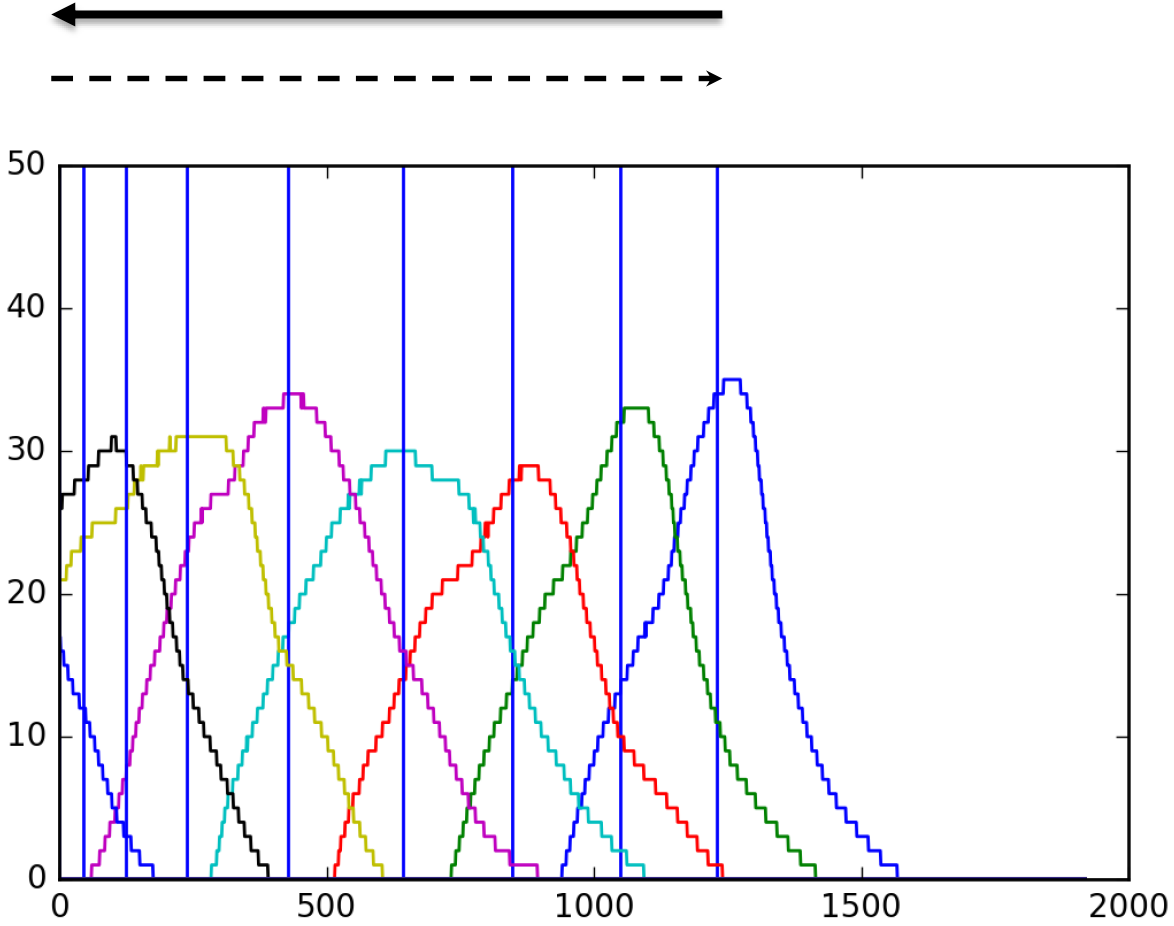
\includegraphics[angle=0,width=14cm]{handcontrol/Bilder/histogramm_schwerpunkt.png}
\caption{Histogramme der Differenzbilder mit Schwerpunkt}
\end{figure}

\section{Entwicklung des Algorithmus}
Der Algorithmus wurde als erstes in MATLAB mit aufgenommenen Videos entwickelt. Nachher wurde auf Python mit OpenCV Binding umgestellt, um einen besseren Vergleich mit der C++ Version zu gewährleisten. Als IDE für Python wurde \href{https://github.com/spyder-ide/spyder}{Spyder} mit dem \href{https://www.continuum.io/downloads}{Anaconda Framework} verwendet. Um den Algorithmus separat von der App zu entwickeln wurde ein "`test\_handcontrol.pro"' Projekt erstellt, welches als eine Art Modultest fungiert. Zu finden in dem schon am Anfang des Kapitels genannten Verzeichnis in Github.

\section{Verbesserungen}
Die Verbesserungen zum Auslesen der Kamera wurden schon in einem separaten Abschnitt behandelt. Für den Algorithmus könnte man statt Grauwertbilder auch Bilder aus dem HSV Raum verwenden. Dort könnte man ggf. Helligkeitsveränderung besser abfangen. Außerdem kann es manchmal vorkommen, dass mehrfach Erkennung erfolgen, diese könnten durch einen Timer abgefangen werden. Eine Verschiebung der Berechnung zur Grafikkarte mittels OpenGL oder OpenCL, wie vorher schon erwähnt, könnte die CPU entlasten und ganz andere Möglichkeiten der Analyse des Frames bieten. Bei der Differenzbildung der Frames entstehen positive und negative Abweichungen, diese könnten in einem verbesserten Algo. separat berücksichtigt werden.

